\documentclass{beamer}

\usepackage{tikz}
\usetikzlibrary{calc}
\usetikzlibrary{math}
\usetikzlibrary{arrows.meta}
\usetikzlibrary{positioning}
\usetikzlibrary{shapes.multipart}
\usepackage{pgfplots}
\usepgfplotslibrary{dateplot}
\pgfplotscreateplotcyclelist{rainbow}{
	{red,mark=*},
	{orange,mark=*},
	{yellow!75!black,mark=*},
	{green!50!black,mark=*},
	{blue,mark=*},
	{purple!50!black,mark=*}%
}
\pgfplotscreateplotcyclelist{rainbow2}{
	{red,mark=*},
	{blue,mark=*}%
}
\pgfplotscreateplotcyclelist{rainbow3}{
	{red,mark=*},
	{green!50!black,mark=*},
	{blue,mark=*}%
}
\pgfplotscreateplotcyclelist{rainbow4}{
	{red,mark=*},
	{orange,mark=*},
	{green!50!black,mark=*},
	{blue,mark=*}%
}
\pgfplotscreateplotcyclelist{rainbow5}{
	{red,mark=*},
	{orange,mark=*},
	{yellow!75!black,mark=*},
	{green!50!black,mark=*},
	{blue,mark=*}%
}
\pgfplotscreateplotcyclelist{rainbow6}{
	{red,mark=*},
	{orange,mark=*},
	{yellow!75!black,mark=*},
	{green!50!black,mark=*},
	{blue,mark=*},
	{purple!50!black,mark=*}%
}
\usepackage{ifthen}
\tikzset{>={Stealth[length=2mm]}}
\newcommand{\todocite}{{\color{red}CITE}}
\newcommand{\todo}[1]{{\color{red}TODO: #1}}
\usepackage{float}
\usepackage{siunitx}
\sisetup{per-mode=symbol}
\newcommand{\pfrac}[2]{\left(\frac{#1}{#2}\right)}
\usepackage{subcaption}
\usepackage[defaultlines=3,all]{nowidow}

\usepackage{multicol}
\usepackage{listings}
\lstset{
	basicstyle=\tiny\ttfamily\color{blue!50!black},
	keywordstyle=\color{purple},
	identifierstyle=\color{black},
	stringstyle=\color{green!50!black},
	showstringspaces=false,
	commentstyle=\color{gray},
	tabsize=2,
	gobble=4
}
\usepackage{biblatex}
\addbibresource{bibfile.bib}

\setbeameroption{show notes on second screen=right}
\day=12\relax
\month=06\relax
\year=2025\relax

\AtBeginSection[] {
	\begin{frame}
		\frametitle{Table of Contents}
		\tableofcontents[currentsection]
	\end{frame}
}
\AtBeginSubsection[] {
	\begin{frame}
		\frametitle{Table of Contents}
		\tableofcontents[currentsubsection]
	\end{frame}
}

\title{Evaluating HLS for FPGA-Based Database Engines%
}
\author{Clarity Shimoniak}
\institute[UCR]{University of California, Riverside}
\date{2025}


\begin{document}

\frame{\titlepage}

\begin{frame}
	\frametitle{Table of Contents}
	\tableofcontents
\end{frame}


\section{Motivation}

\begin{frame}
	\frametitle{Hardware Limitations}
	\note[item]{
		These are the same slides that have come at the beginning of half of my
		classes in the last few years, so I'll keep this brief
	}
	\begin{columns}
		\column{0.47\linewidth}
		\begin{itemize}
			\item Demand for computation is increasing
			\item Demand for data storage is increasing
			\item Silicon's physical properties are limited
			\begin{itemize}
				\item Clock speeds cannot increase further
			\end{itemize}
			\item Parallelism is the only route forward
		\end{itemize}

		\column{0.5\linewidth}
		\begin{figure}
			\centering
			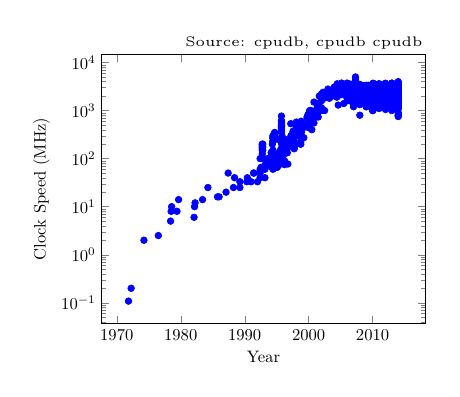
\begin{tikzpicture}[scale=0.6]
	\node[anchor=south east] at (7, 5.6)
		{\tiny Source: {\citetitle{cpudb}, \citeyear{cpudb} \autocite{cpudb}}};
	\begin{axis}
		[
			xlabel={Year},
			ylabel={Clock Speed ($\unit{\mega\hertz}$)},
			date coordinates in=x,
			xticklabel={\year},
			xtick={
				1970-01-01,
				1980-01-01,
				1990-01-01,
				2000-01-01,
				2010-01-01
			},
			ymode=log,
		]
		\addplot[only marks, color=blue] coordinates {
			(2002-01-01, 1700)
			(2005-01-04, 3200)
			(2006-01-01, 3460)
			(2006-01-01, 3730)
			(2007-01-01, 1600)
			(2007-01-04, 1600)
			(2007-01-04, 1800)
			(2007-01-04, 1730)
			(2006-01-07, 2160)
			(2007-01-01, 1600)
			(2007-01-01, 1830)
			(2007-01-04, 1860)
			(2007-01-07, 1860)
			(2007-01-07, 2400)
			(2007-01-07, 2930)
			(2007-01-07, 2000)
			(2007-01-07, 1600)
			(2007-01-07, 2130)
			(2007-01-07, 2400)
			(2007-01-07, 2400)
			(2007-01-07, 2930)
			(2007-01-07, 2000)
			(2007-01-07, 1860)
			(2008-01-01, 2400)
			(2007-01-10, 1460)
			(2007-01-10, 1600)
			(2007-01-10, 2800)
			(2008-01-07, 2660)
			(2007-01-01, 1730)
			(2007-01-10, 1200)
			(2008-01-01, 1600)
			(2008-01-01, 1730)
			(2009-01-04, 2400)
			(2008-01-04, 2000)
			(2008-01-07, 2200)
			(2008-01-04, 1860)
			(2008-01-04, 800)
			(2008-01-10, 2160)
			(2008-01-04, 2260)
			(2008-01-07, 2160)
			(2008-01-01, 2400)
			(2008-01-07, 3400)
			(2008-01-07, 2130)
			(2008-01-07, 2130)
			(2008-01-07, 2130)
			(2008-01-07, 2400)
			(2008-01-07, 2400)
			(2008-01-07, 2130)
			(2008-01-07, 2660)
			(2008-01-10, 1830)
			(2008-01-10, 2660)
			(2008-01-10, 2930)
			(2009-01-04, 3060)
			(2009-01-10, 3200)
			(2009-01-01, 2000)
			(2008-01-10, 1660)
			(2009-01-01, 2700)
			(2009-01-01, 2130)
			(2009-01-10, 2200)
			(2009-01-04, 1200)
			(2009-01-04, 2000)
			(2010-01-01, 2800)
			(2009-01-07, 2930)
			(2010-01-01, 2530)
			(2010-01-01, 2800)
			(2009-01-04, 2800)
			(2009-01-01, 2200)
			(2009-01-07, 2400)
			(2010-01-07, 2100)
			(2010-01-07, 2700)
			(2010-01-01, 1460)
			(2010-01-04, 2800)
			(2010-01-07, 3000)
			(2010-01-10, 3200)
			(2009-01-07, 2930)
			(2010-01-01, 3060)
			(2010-01-04, 3200)
			(2010-01-07, 3330)
			(2010-01-01, 2400)
			(2010-01-01, 2300)
			(2009-01-07, 1600)
			(2009-01-07, 1730)
			(2010-01-07, 1860)
			(2009-01-07, 2000)
			(2010-01-07, 2130)
			(2010-01-01, 1600)
			(2010-01-01, 1330)
			(2010-01-01, 1600)
			(2010-01-01, 1730)
			(2010-01-01, 2260)
			(2010-01-01, 2260)
			(2010-01-01, 2530)
			(2010-01-01, 3200)
			(2010-01-01, 3330)
			(2010-01-01, 3460)
			(2010-01-01, 2000)
			(2010-01-01, 1060)
			(2010-01-01, 2130)
			(2011-01-07, 2800)
			(2010-01-01, 1830)
			(2010-01-01, 2930)
			(2011-01-01, 2933)
			(2010-01-01, 1730)
			(2010-01-01, 2000)
			(2010-01-01, 1866)
			(2010-01-01, 1866)
			(2010-01-01, 2000)
			(2010-01-01, 1866)
			(2010-01-01, 1866)
			(2010-01-01, 2000)
			(2010-01-01, 2666)
			(2010-01-01, 2000)
			(2010-01-01, 2266)
			(2010-01-01, 2000)
			(2010-01-01, 1066)
			(2010-01-01, 2130)
			(2010-01-01, 1200)
			(2010-01-01, 3330)
			(2010-01-07, 3200)
			(2010-01-07, 2800)
			(2010-01-04, 2660)
			(2010-01-04, 2930)
			(2010-01-04, 3060)
			(2010-01-04, 3600)
			(2010-01-04, 3200)
			(2010-01-04, 3200)
			(2010-01-07, 2400)
			(2010-01-04, 1200)
			(2010-01-04, 2400)
			(2010-01-04, 1200)
			(2010-01-07, 1730)
			(2010-01-04, 1860)
			(2010-01-04, 1200)
			(2010-01-04, 1060)
			(2010-01-04, 1330)
			(2010-01-04, 1200)
			(2010-01-04, 1830)
			(2010-01-07, 2660)
			(2010-01-07, 2660)
			(2010-01-07, 2260)
			(2010-01-04, 1200)
			(2010-01-04, 1600)
			(2010-01-04, 1900)
			(2010-01-07, 1460)
			(2010-01-07, 1330)
			(2010-01-07, 2800)
			(2010-01-04, 2130)
			(2004-01-04, 2400)
			(2010-01-10, 1330)
			(2010-01-10, 1330)
			(2011-01-01, 1330)
			(2011-01-01, 1200)
			(2010-01-07, 1500)
			(2010-01-07, 2000)
			(2010-01-07, 2130)
			(2010-01-07, 3330)
			(2010-01-07, 2530)
			(2010-01-07, 2530)
			(2011-01-01, 2270)
			(2011-01-01, 2500)
			(2011-01-01, 3300)
			(2011-01-01, 2700)
			(2011-01-01, 2300)
			(2011-01-01, 3400)
			(2011-01-01, 2800)
			(2011-01-01, 2000)
			(2011-01-01, 2100)
			(2011-01-01, 2300)
			(2011-01-01, 2300)
			(2011-01-01, 2500)
			(2011-01-01, 2700)
			(2011-01-01, 2500)
			(2011-01-04, 3100)
			(2011-01-04, 3200)
			(2011-01-04, 3200)
			(2011-01-04, 3300)
			(2011-01-04, 3300)
			(2011-01-04, 2400)
			(2011-01-04, 3400)
			(2011-01-04, 3500)
			(2010-01-07, 2000)
			(2011-01-01, 3460)
			(2011-01-01, 3060)
			(2011-01-01, 3600)
			(2011-01-01, 3200)
			(2011-01-01, 2930)
			(2011-01-01, 2530)
			(2011-01-01, 2260)
			(2011-01-01, 2130)
			(2011-01-01, 1600)
			(2011-01-01, 3460)
			(2011-01-01, 3460)
			(2011-01-01, 2660)
			(2011-01-01, 2660)
			(2011-01-04, 2200)
			(2011-01-07, 2400)
			(2011-01-07, 2000)
			(2012-01-04, 2100)
			(2012-01-04, 2600)
			(2011-01-01, 3100)
			(2011-01-01, 2500)
			(2011-01-04, 3100)
			(2011-01-07, 2600)
			(2011-01-07, 3400)
			(2011-01-04, 2100)
			(2011-01-04, 2200)
			(2011-01-10, 2300)
			(2012-01-01, 2400)
			(2011-01-04, 2900)
			(2011-01-07, 3000)
			(2011-01-01, 2700)
			(2011-01-10, 2400)
			(2012-01-01, 2500)
			(2011-01-01, 2000)
			(2011-01-10, 2800)
			(2011-01-10, 2200)
			(2011-01-10, 2200)
			(2011-01-10, 2400)
			(2011-01-10, 2500)
			(2011-01-10, 2700)
			(2011-01-04, 2600)
			(2011-01-04, 2200)
			(2011-01-04, 2600)
			(2011-01-07, 2700)
			(2011-01-07, 2300)
			(2011-01-07, 2700)
			(2012-01-04, 2800)
			(2012-01-04, 2400)
			(2011-01-04, 2800)
			(2011-01-07, 3000)
			(2012-01-04, 3100)
			(2011-01-04, 1730)
			(2011-01-04, 1860)
			(2011-01-04, 2260)
			(2011-01-04, 2260)
			(2011-01-04, 2260)
			(2011-01-04, 2000)
			(2011-01-04, 2000)
			(2011-01-04, 2000)
			(2011-01-04, 2660)
			(2011-01-04, 2130)
			(2011-01-04, 2400)
			(2011-01-04, 2400)
			(2011-01-04, 2400)
			(2011-01-04, 2000)
			(2011-01-04, 2130)
			(2011-01-04, 2000)
			(2011-01-04, 2130)
			(2011-01-04, 2130)
			(2011-01-01, 1400)
			(2011-01-01, 2300)
			(2011-01-01, 2100)
			(2011-01-01, 2300)
			(2011-01-01, 1600)
			(2011-01-01, 1500)
			(2011-01-04, 1800)
			(2011-01-04, 1700)
			(2011-01-01, 1400)
			(2011-01-04, 1700)
			(2011-01-04, 1300)
			(2011-01-04, 2500)
			(2011-01-04, 3100)
			(2011-01-07, 3600)
			(2011-01-04, 2000)
			(2011-01-04, 2100)
			(2011-01-04, 1200)
			(2011-01-01, 1660)
			(2011-01-04, 1100)
			(2011-01-04, 1600)
			(2011-01-04, 3330)
			(2011-01-07, 1600)
			(2011-01-07, 3300)
			(2011-01-07, 1600)
			(2011-01-04, 1500)
			(2011-01-07, 1300)
			(2011-01-07, 1200)
			(2011-01-07, 1860)
			(2011-01-07, 2130)
			(2011-01-10, 1400)
			(2011-01-07, 1900)
			(2011-01-10, 1300)
			(2011-01-10, 2200)
			(2011-01-10, 2400)
			(2011-01-10, 3200)
			(2012-01-01, 3600)
			(2011-01-10, 1800)
			(2012-01-01, 2300)
			(2012-01-01, 1400)
			(2012-01-01, 1400)
			(2012-01-01, 1300)
			(2012-01-01, 1600)
			(2012-01-01, 1700)
			(2012-01-01, 3100)
			(2012-01-01, 2700)
			(2012-01-01, 2200)
			(2012-01-01, 1800)
			(2012-01-01, 2000)
			(2012-01-01, 3300)
			(2012-01-01, 2400)
			(2012-01-01, 2900)
			(2012-01-01, 2000)
			(2012-01-01, 2500)
			(2012-01-01, 1800)
			(2012-01-01, 2300)
			(2012-01-01, 2600)
			(2012-01-01, 2900)
			(2012-01-01, 2400)
			(2012-01-01, 3000)
			(2012-01-01, 3200)
			(2012-01-04, 2400)
			(2012-01-04, 2400)
			(2012-01-04, 2200)
			(2012-01-04, 2600)
			(2012-01-04, 2200)
			(2012-01-04, 2900)
			(2012-01-04, 2000)
			(2012-01-04, 1800)
			(2012-01-04, 2100)
			(2012-01-04, 2400)
			(2012-01-04, 2000)
			(2012-01-04, 2200)
			(2012-01-04, 1800)
			(2012-01-04, 1900)
			(2012-01-01, 3300)
			(2012-01-01, 3600)
			(2012-01-04, 2700)
			(2012-01-04, 2300)
			(2012-01-01, 3200)
			(2012-01-01, 3100)
			(2012-01-04, 2900)
			(2012-01-04, 2700)
			(2012-01-04, 2600)
			(2012-01-04, 2900)
			(2012-01-04, 2800)
			(2012-01-04, 2600)
			(2012-01-04, 2000)
			(2012-01-04, 2300)
			(2012-01-04, 2300)
			(2012-01-04, 2100)
			(2012-01-04, 1800)
			(2012-01-04, 3100)
			(2012-01-04, 2800)
			(2012-01-04, 2900)
			(2012-01-04, 3300)
			(2012-01-04, 3400)
			(2012-01-04, 2300)
			(2012-01-04, 3500)
			(2012-01-04, 3100)
			(2012-01-04, 2500)
			(2012-01-01, 3400)
			(2012-01-04, 1800)
			(2012-01-04, 2400)
			(2012-01-04, 3100)
			(2012-01-04, 3400)
			(2012-01-04, 2900)
			(2012-01-04, 1700)
			(2012-01-04, 2500)
			(2012-01-04, 1900)
			(2012-01-04, 3700)
			(2012-01-04, 3600)
			(2012-01-04, 3500)
			(2012-01-04, 2500)
			(2012-01-04, 3400)
			(2012-01-04, 3400)
			(2012-01-04, 3300)
			(2012-01-04, 3100)
			(2012-01-04, 2300)
			(2012-01-04, 1800)
			(2012-01-04, 2600)
			(2012-01-04, 1500)
			(1993-03-01, 40)
			(1999-11-29, 600)
			(1999-11-01, 750)
			(2000-05-01, 1000)
			(2001-06-01, 1400)
			(2004-06-01, 2600)
			(2005-06-01, 2800)
			(2006-01-01, 2600)
			(2006-07-01, 2800)
			(2005-05-31, 2200)
			(2006-06-01, 2600)
			(2007-02-01, 3100)
			(2007-08-01, 3200)
			(2007-08-20, 1600)
			(2008-10-01, 2100)
			(2008-12-01, 2500)
			(2002-06-01, 1800)
			(2003-02-01, 2167)
			(1996-03-27, 75)
			(1996-03-27, 90)
			(1997-04-01, 233)
			(1998-04-01, 300)
			(1998-05-01, 333)
			(1998-11-01, 400)
			(1998-11-01, 500)
			(1999-02-01, 450)
			(2003-04-01, 1800)
			(2003-09-01, 2000)
			(2006-08-01, 2600)
			(2008-04-01, 2100)
			(2008-04-01, 2200)
			(2008-04-01, 2300)
			(2006-08-01, 1800)
			(2006-08-01, 2000)
			(2006-08-01, 2200)
			(2006-08-01, 2400)
			(2006-08-01, 2600)
			(2007-02-01, 2800)
			(2007-08-01, 3000)
			(2007-09-01, 2000)
			(2008-04-01, 2300)
			(2008-11-01, 2700)
			(2009-04-01, 2900)
			(2009-06-01, 2600)
			(2007-02-01, 2800)
			(2007-08-05, 3000)
			(2007-09-10, 2000)
			(2006-08-01, 2800)
			(2007-04-01, 3000)
			(2008-04-01, 2500)
			(2009-07-01, 2800)
			(2009-02-01, 2600)
			(2009-02-01, 2800)
			(2009-02-01, 2500)
			(2009-02-01, 2600)
			(2009-02-01, 2600)
			(2009-01-01, 2800)
			(2009-05-01, 2800)
			(2009-01-01, 3000)
			(2009-08-01, 3200)
			(2008-04-01, 2400)
			(2008-03-27, 2400)
			(2008-07-01, 2500)
			(2008-07-01, 2600)
			(2008-07-01, 2000)
			(2005-08-01, 2200)
			(2007-06-01, 2000)
			(1990-06-01, 40)
			(1993-01-01, 100)
			(1992-01-01, 33)
			(1995-06-01, 120)
			(1996-02-01, 120)
			(1997-05-01, 188)
			(2000-02-01, 450)
			(1992-10-01, 100)
			(1992-10-01, 125)
			(1992-10-01, 150)
			(1992-10-01, 166)
			(1992-10-01, 175)
			(1992-10-01, 190)
			(1992-10-01, 200)
			(1994-06-01, 225)
			(1994-06-01, 233)
			(1994-06-01, 266)
			(1994-06-01, 275)
			(1994-06-01, 300)
			(1995-09-01, 231)
			(1995-09-01, 233)
			(1995-09-01, 99)
			(1994-09-07, 250)
			(1994-09-07, 266)
			(1994-09-07, 291)
			(1994-09-07, 300)
			(1994-09-07, 333)
			(1994-09-07, 350)
			(1995-10-01, 352)
			(1995-10-01, 374)
			(1995-10-01, 400)
			(1995-10-01, 433)
			(1995-10-01, 437)
			(1995-10-01, 466)
			(1995-10-01, 480)
			(1995-10-01, 500)
			(1995-10-01, 533)
			(1995-10-01, 600)
			(1995-10-01, 612)
			(1995-10-01, 767)
			(1997-03-17, 533)
			(1998-11-01, 600)
			(1998-02-01, 466)
			(1998-02-01, 500)
			(1998-02-01, 525)
			(1998-02-01, 575)
			(1999-12-01, 616)
			(1999-12-01, 667)
			(1999-12-01, 700)
			(1999-12-01, 731)
			(1999-12-01, 750)
			(1999-12-01, 833)
			(2001-02-01, 833)
			(2001-06-01, 1000)
			(2001-06-01, 1224)
			(2001-06-01, 1250)
			(2002-01-01, 1000)
			(2002-01-01, 1150)
			(2004-08-16, 1300)
			(1995-06-01, 110)
			(1994-06-01, 60)
			(1994-06-01, 70)
			(1994-06-01, 85)
			(1999-04-01, 272)
			(1998-05-01, 360)
			(1999-05-01, 450)
			(2008-07-01, 2520)
			(2008-07-01, 2750)
			(1996-09-01, 170)
			(1995-10-01, 101)
			(1995-10-01, 118)
			(1994-06-01, 120)
			(1996-09-01, 132)
			(1996-09-01, 160)
			(1996-09-01, 180)
			(1995-11-02, 160)
			(1995-11-02, 180)
			(1998-09-01, 440)
			(2000-01-01, 440)
			(2000-01-01, 500)
			(2000-01-01, 550)
			(2000-11-01, 552)
			(2001-05-01, 750)
			(1997-10-01, 160)
			(1996-10-01, 77)
			(1998-10-05, 200)
			(1998-10-05, 222)
			(1998-10-05, 375)
			(2001-01-01, 1000)
			(2004-06-01, 1900)
			(2007-05-01, 3500)
			(2007-05-01, 3800)
			(2007-05-01, 4200)
			(2007-05-01, 4700)
			(2007-05-01, 5000)
			(2010-02-01, 3550)
			(2010-02-01, 3700)
			(1997-08-01, 266)
			(1998-10-01, 400)
			(1995-02-01, 66)
			(1993-09-01, 80)
			(1995-07-01, 133)
			(1998-10-01, 200)
			(1993-04-01, 66)
			(1993-04-01, 75)
			(1995-06-01, 120)
			(1995-02-01, 66)
			(1995-10-01, 100)
			(1996-05-01, 200)
			(1997-04-01, 300)
			(1994-12-01, 100)
			(1996-07-01, 166)
			(1996-07-01, 200)
			(1996-07-01, 225)
			(1996-07-01, 233)
			(1996-07-01, 250)
			(1997-08-01, 300)
			(1997-08-01, 320)
			(1997-08-01, 332)
			(1997-08-01, 350)
			(1997-08-01, 360)
			(1997-08-01, 375)
			(1971-11-01, 0.108)
			(1972-04-01, 0.2)
			(1974-04-01, 2)
			(1978-06-01, 5)
			(1978-07-01, 8)
			(1978-08-01, 10)
			(1979-06-01, 8)
			(1982-02-01, 6)
			(1982-03-01, 10)
			(1982-04-01, 12)
			(1985-10-01, 16)
			(1987-02-01, 20)
			(1988-04-01, 25)
			(1989-04-01, 33)
			(1989-04-01, 25)
			(1990-05-01, 33)
			(1991-06-01, 50)
			(1992-08-01, 66)
			(1994-03-01, 100)
			(2008-01-04, 1600)
			(2008-01-07, 1600)
			(2009-12-21, 1667)
			(2010-09-14, 1300)
			(2010-11-22, 1300)
			(2008-06-03, 1600)
			(2009-01-01, 1660)
			(2009-12-21, 1666)
			(2008-01-04, 1330)
			(2008-04-02, 1600)
			(1998-08-01, 300)
			(2009-01-07, 2400)
			(2009-01-07, 2500)
			(2009-01-07, 1200)
			(2008-01-01, 2130)
			(2007-01-01, 1800)
			(2007-07-01, 2200)
			(2007-10-01, 2400)
			(2006-07-01, 1860)
			(2006-07-01, 2133)
			(2006-07-01, 2400)
			(2006-07-01, 2660)
			(2007-07-01, 2666)
			(2007-07-01, 3000)
			(2008-04-01, 2530)
			(2008-08-01, 2660)
			(2008-10-01, 2800)
			(2009-01-01, 2930)
			(2009-05-01, 3060)
			(2008-01-01, 2660)
			(2008-01-01, 3000)
			(2008-01-01, 3160)
			(2008-08-01, 3330)
			(2008-06-01, 2266)
			(2008-06-13, 2400)
			(2008-09-01, 1400)
			(2008-05-01, 1800)
			(2006-08-01, 2167)
			(2006-08-28, 1667)
			(2006-08-28, 2000)
			(2006-08-01, 2330)
			(2007-05-01, 2400)
			(2007-09-01, 2600)
			(2008-07-01, 2533)
			(2008-01-01, 2600)
			(2009-04-01, 3060)
			(2006-07-01, 2930)
			(2007-08-01, 2800)
			(2008-01-01, 2800)
			(2007-01-01, 2400)
			(2007-04-01, 2667)
			(2008-08-01, 2330)
			(2008-11-01, 2500)
			(2009-04-01, 2660)
			(2008-03-01, 2500)
			(2008-08-01, 2666)
			(2008-03-01, 2660)
			(2008-03-01, 2830)
			(2008-08-01, 3000)
			(2006-08-01, 2667)
			(2007-04-01, 2933)
			(2007-07-01, 3000)
			(2008-08-01, 2530)
			(2007-11-01, 3000)
			(2008-03-01, 3200)
			(2009-04-01, 1400)
			(2006-01-01, 1830)
			(2006-01-01, 2167)
			(2006-06-01, 2330)
			(2010-01-07, 2130)
			(2010-09-26, 2530)
			(2010-01-01, 2933)
			(2010-01-01, 3067)
			(2010-05-01, 3200)
			(2010-08-01, 3333)
			(2010-09-26, 2530)
			(2010-09-26, 2667)
			(2010-01-01, 3200)
			(2010-01-01, 3333)
			(2010-01-01, 3333)
			(2010-01-01, 3467)
			(2010-04-01, 3600)
			(2009-09-01, 2667)
			(2010-01-01, 2400)
			(2009-09-23, 1600)
			(2009-09-01, 2800)
			(2009-09-01, 2933)
			(2008-11-01, 2667)
			(2008-11-01, 2933)
			(2009-05-01, 3060)
			(2008-11-01, 3200)
			(2009-05-01, 3333)
			(2010-01-01, 2533)
			(2008-10-01, 3200)
			(2009-05-01, 3333)
			(2010-03-01, 3333)
			(2011-01-09, 3400)
			(2001-05-01, 800)
			(2002-07-01, 1000)
			(2007-01-04, 1600)
			(2007-06-01, 1800)
			(2007-01-10, 2200)
			(2008-01-07, 2500)
			(2008-11-01, 2600)
			(2010-01-01, 2800)
			(1994-07-01, 100)
			(1995-03-01, 120)
			(1995-06-01, 133)
			(1996-06-01, 166)
			(1996-06-01, 200)
			(1993-03-01, 60)
			(1993-03-01, 66)
			(2009-05-01, 1300)
			(2004-06-21, 3600)
			(2000-11-01, 1500)
			(2001-09-01, 2000)
			(2002-01-01, 2200)
			(2002-04-02, 2400)
			(2005-02-21, 3733)
			(2005-12-01, 2660)
			(2006-01-01, 2800)
			(2006-10-01, 3000)
			(2006-01-01, 3000)
			(2006-01-01, 3200)
			(2006-07-01, 3400)
			(2006-01-01, 3400)
			(2006-05-01, 3600)
			(1997-05-01, 300)
			(1998-01-01, 333)
			(2000-03-01, 1000)
			(1999-02-01, 500)
			(1999-10-01, 733)
			(1997-01-01, 200)
			(1997-06-01, 233)
			(1995-11-01, 200)
			(2007-01-01, 1860)
			(2007-01-01, 2130)
			(2007-10-01, 2400)
			(2007-01-10, 2330)
			(2007-10-01, 2660)
			(2007-10-01, 2660)
			(2007-10-01, 3000)
			(2006-06-01, 1600)
			(2006-06-01, 1860)
			(2006-06-01, 2000)
			(2006-06-01, 2333)
			(2006-06-01, 2660)
			(2006-06-01, 3000)
			(2006-08-01, 2600)
			(2006-08-01, 3000)
			(2006-08-01, 3200)
			(2006-08-01, 3400)
			(2008-01-01, 3000)
			(2008-01-07, 3160)
			(2007-01-10, 1860)
			(2006-01-10, 1600)
			(2006-01-10, 1860)
			(2006-12-01, 2000)
			(2006-11-01, 2330)
			(2007-01-10, 2000)
			(2007-01-10, 2330)
			(2007-01-10, 2500)
			(2007-01-10, 2660)
			(2007-11-01, 2830)
			(2007-01-10, 3000)
			(2007-01-10, 3000)
			(2009-01-01, 1860)
			(2010-01-01, 2000)
			(2009-03-01, 2000)
			(2009-01-01, 2130)
			(2010-01-01, 2260)
			(2009-01-01, 2260)
			(2009-01-01, 2400)
			(2009-03-01, 2530)
			(2010-03-01, 2400)
			(2010-01-01, 2530)
			(2010-03-01, 2670)
			(2010-02-10, 2533)
			(2009-01-01, 3000)
			(2009-01-01, 2830)
			(2010-01-01, 2260)
			(2009-01-07, 1860)
			(2008-01-07, 1860)
			(2008-01-04, 3000)
			(2007-01-01, 1860)
			(2008-02-27, 2133)
			(2008-03-01, 2330)
			(2008-01-01, 2500)
			(2009-01-01, 2260)
			(2010-01-01, 1860)
			(2010-01-01, 2130)
			(2010-01-01, 2260)
			(2009-01-01, 2400)
			(2009-01-01, 2530)
			(2009-01-01, 2660)
			(2009-01-01, 2930)
			(2009-01-07, 3060)
			(2009-01-10, 3200)
			(2009-01-01, 3200)
			(2009-01-07, 3330)
			(2010-01-07, 3200)
			(2010-01-01, 3330)
			(2009-01-01, 3200)
			(2009-01-07, 3330)
			(2007-01-01, 2130)
			(2007-01-01, 2400)
			(2007-01-07, 2660)
			(2008-01-01, 2500)
			(2008-01-07, 2660)
			(2008-01-01, 2660)
			(2008-01-01, 2830)
			(2008-01-07, 3000)
			(2009-01-01, 3160)
			(2009-09-01, 2400)
			(2009-01-07, 2530)
			(2009-09-01, 2667)
			(2009-01-07, 2800)
			(2009-01-07, 2930)
			(2010-01-04, 3060)
			(2007-01-10, 3330)
			(2008-01-07, 3500)
			(2007-01-10, 3400)
			(2006-01-10, 2660)
			(2007-01-07, 3000)
			(2007-01-10, 3000)
			(2007-01-10, 3160)
			(2008-01-07, 3330)
			(2007-01-10, 3000)
			(2007-01-10, 3200)
			(2009-03-01, 2670)
			(2009-01-01, 2800)
			(2009-01-01, 2930)
			(2010-01-01, 2660)
			(2010-01-01, 2800)
			(2010-01-01, 3060)
			(2010-01-01, 2930)
			(2010-01-01, 3460)
			(2010-01-01, 3330)
			(1996-01-01, 180)
			(1996-01-01, 195)
			(1996-01-01, 196)
			(1996-01-01, 200)
			(1996-01-01, 250)
			(1986-01-01, 16)
			(1988-06-01, 40)
			(1992-06-01, 100)
			(1995-07-01, 240)
			(1994-05-01, 200)
			(1995-07-01, 250)
			(1992-11-01, 100)
			(1992-11-01, 150)
			(1992-11-01, 175)
			(1992-11-01, 200)
			(1993-08-01, 100)
			(1994-03-01, 133)
			(1994-06-01, 150)
			(1994-03-01, 133)
			(1996-01-01, 150)
			(1996-01-01, 180)
			(1996-01-01, 200)
			(1996-01-01, 250)
			(1994-06-07, 75)
			(1994-06-07, 75)
			(1979-09-01, 14)
			(1983-06-01, 14)
			(1984-04-01, 25)
			(1987-06-01, 50)
			(1991-01-01, 33)
			(1994-04-01, 66)
			(1999-08-01, 500)
			(2001-07-01, 733)
			(1994-03-01, 93)
			(1994-06-01, 100)
			(1994-06-01, 125)
			(1995-08-01, 150)
			(1993-06-01, 72)
			(1998-11-01, 270)
			(1998-11-01, 300)
			(1998-11-01, 350)
			(1998-11-01, 360)
			(2000-07-01, 400)
			(1991-06-01, 50)
			(1992-06-01, 40)
			(1992-06-01, 50)
			(1992-06-01, 60)
			(1995-06-01, 75)
			(1995-06-01, 90)
			(1995-11-01, 143)
			(1995-11-01, 167)
			(1995-11-01, 200)
			(1995-11-01, 248)
			(1995-11-01, 296)
			(2000-09-01, 600)
			(2000-09-01, 750)
			(2000-09-01, 900)
			(2005-07-01, 1400)
			(2007-07-01, 1400)
			(1976-07-01, 2.5)
			(2010-04-01, 1800)
			(1997-10-13, 180)
			(1997-10-14, 200)
			(1997-10-15, 225)
			(2013-01-04, 3500)
			(2013-09-01, 2000)
			(2006-01-07, 2930)
			(2002-01-01, 2000)
			(2003-01-07, 2400)
			(2003-01-10, 2800)
			(2002-01-07, 1600)
			(2006-01-10, 2660)
			(2007-01-04, 2000)
			(2007-01-04, 2930)
			(2007-01-07, 2200)
			(2007-01-07, 2600)
			(2007-01-07, 3000)
			(2007-01-10, 2400)
			(2008-01-01, 2000)
			(2008-01-01, 2600)
			(2008-01-04, 2530)
			(2008-01-07, 2660)
			(2009-01-04, 2200)
			(2009-01-01, 2930)
			(2008-01-07, 2330)
			(2008-01-07, 2400)
			(2009-01-01, 2130)
			(2008-01-07, 2000)
			(2008-01-07, 2260)
			(2008-01-10, 2000)
			(2009-01-01, 2530)
			(2009-01-04, 2660)
			(2008-01-10, 2500)
			(2009-01-01, 2000)
			(2009-01-04, 1800)
			(2009-01-01, 2330)
			(2009-01-04, 3060)
			(2009-01-07, 2260)
			(2009-01-07, 2200)
			(2009-01-04, 2660)
			(2009-01-04, 1300)
			(2009-01-07, 2260)
			(2009-01-04, 2100)
			(2009-01-07, 1300)
			(2011-01-01, 2200)
			(2011-01-01, 2600)
			(2011-01-01, 2800)
			(2011-01-01, 3300)
			(2012-01-07, 2200)
			(2011-01-01, 2300)
			(2010-01-10, 1000)
			(2010-01-10, 1000)
			(2010-01-10, 1300)
			(2010-01-10, 1300)
			(2012-01-04, 1500)
			(2011-01-04, 1500)
			(2011-01-04, 1200)
			(2011-01-10, 1200)
			(2011-01-10, 3500)
			(2012-01-01, 2800)
			(2012-01-01, 3000)
			(2012-01-07, 3000)
			(2012-01-07, 2700)
			(2012-01-07, 3400)
			(2012-01-07, 3300)
			(2012-01-07, 2800)
			(2012-01-07, 2600)
			(2012-01-07, 2900)
			(2012-01-04, 1400)
			(2012-01-07, 1700)
			(2012-01-07, 1500)
			(2012-01-04, 2600)
			(2012-01-04, 2800)
			(2012-01-04, 2800)
			(2012-01-04, 2900)
			(2012-01-04, 3200)
			(2012-01-07, 3100)
			(2012-01-07, 2700)
			(2012-01-07, 2900)
			(2012-01-07, 1600)
			(2012-01-07, 1500)
			(2012-01-10, 2000)
			(2012-01-07, 1900)
			(2012-01-07, 2500)
			(2012-01-04, 2400)
			(2012-01-07, 1800)
			(2012-01-07, 1400)
			(2012-01-07, 2800)
			(2012-01-07, 2700)
			(2012-01-07, 2200)
			(2013-01-01, 3200)
			(2013-01-01, 3200)
			(2013-01-01, 2500)
			(2013-01-01, 2900)
			(2013-01-01, 2800)
			(2013-01-01, 2600)
			(2013-01-01, 2300)
			(2012-01-07, 3000)
			(2013-01-04, 2700)
			(2012-01-07, 1800)
			(2012-01-07, 2400)
			(2013-01-01, 3000)
			(2013-01-01, 2900)
			(2013-01-01, 2700)
			(2013-01-01, 2100)
			(2013-01-01, 1900)
			(2012-01-07, 2400)
			(2012-01-07, 2400)
			(2012-01-07, 2500)
			(2012-01-07, 1800)
			(2012-01-07, 2200)
			(2012-01-10, 2530)
			(2012-01-10, 2400)
			(2012-01-10, 2130)
			(2012-01-10, 1730)
			(2012-01-10, 1053)
			(2013-01-01, 2100)
			(2013-01-01, 1800)
			(2013-01-01, 1400)
			(2013-01-01, 1500)
			(2013-01-01, 1500)
			(2013-01-01, 1500)
			(2013-01-01, 1100)
			(2013-01-01, 2000)
			(2013-01-01, 1800)
			(2013-01-01, 2600)
			(2013-01-01, 1900)
			(2013-01-01, 2600)
			(2013-01-01, 2500)
			(2013-01-01, 1800)
			(2013-01-01, 1500)
			(2013-01-01, 1500)
			(2013-01-04, 2000)
			(2013-01-01, 2300)
			(2013-01-04, 3500)
			(2013-01-04, 3000)
			(2013-01-04, 3400)
			(2013-01-04, 3300)
			(2013-01-04, 2600)
			(2013-01-04, 3000)
			(2013-01-10, 2800)
			(2013-01-07, 1300)
			(2013-01-07, 1400)
			(2013-01-04, 3000)
			(2013-01-04, 2700)
			(2013-01-07, 3100)
			(2013-01-07, 2800)
			(2013-01-04, 3200)
			(2013-01-04, 2900)
			(2013-01-04, 3400)
			(2013-01-04, 3400)
			(2013-01-04, 3100)
			(2013-01-04, 2300)
			(2013-01-07, 1100)
			(2013-01-04, 3100)
			(2013-01-04, 1800)
			(2013-01-04, 3300)
			(2013-01-04, 3400)
			(2013-01-04, 3600)
			(2013-01-04, 1000)
			(2013-01-10, 2400)
			(2013-01-07, 1700)
			(2013-01-07, 1800)
			(2013-01-07, 1500)
			(2013-01-04, 2400)
			(2013-01-04, 2400)
			(2013-01-04, 2200)
			(2013-01-04, 2200)
			(2013-01-04, 2000)
			(2013-01-04, 3400)
			(2013-01-04, 3500)
			(2013-01-04, 2500)
			(2013-01-04, 2700)
			(2013-01-04, 2800)
			(2013-01-04, 3000)
			(2013-01-07, 1900)
			(2013-01-07, 1600)
			(2013-01-07, 1900)
			(2013-01-07, 1600)
			(2013-01-07, 1800)
			(2013-01-04, 3400)
			(2013-01-04, 2500)
			(2013-01-04, 3600)
			(2013-01-04, 3100)
			(2013-01-07, 1400)
			(2013-01-04, 1100)
			(2013-01-04, 1100)
			(2013-01-04, 1238)
			(2013-01-04, 1238)
			(2013-01-04, 1053)
			(2013-01-07, 1400)
			(2013-01-07, 1300)
			(2013-01-07, 2000)
			(2013-01-07, 2400)
			(2013-01-07, 2600)
			(2013-01-07, 2800)
			(2013-01-07, 2400)
			(2013-01-07, 2300)
			(2013-01-07, 2000)
			(2013-01-10, 2600)
			(2013-01-07, 2400)
			(2013-01-07, 1800)
			(2013-01-07, 1600)
			(2013-01-07, 3100)
			(2013-01-07, 2800)
			(2013-01-07, 2800)
			(2013-01-07, 2400)
			(2013-01-10, 2500)
			(2013-01-10, 2600)
			(2013-01-10, 2500)
			(2013-01-10, 2900)
			(2013-01-07, 2410)
			(2013-01-07, 2000)
			(2013-01-07, 2410)
			(2013-01-07, 1500)
			(2013-01-07, 1500)
			(2013-01-07, 1600)
			(2013-01-07, 1500)
			(2013-01-07, 1600)
			(2013-01-07, 1600)
			(2013-01-07, 2100)
			(2013-01-07, 1700)
			(2013-01-07, 1700)
			(2013-01-07, 1200)
			(2013-01-04, 2700)
			(2013-01-04, 3000)
			(2013-01-04, 3200)
			(2013-01-10, 2800)
			(2013-01-07, 2000)
			(2013-01-07, 1600)
			(2013-01-07, 2000)
			(2013-01-07, 1460)
			(2013-01-07, 1330)
			(2013-01-07, 1460)
			(2013-01-10, 2000)
			(2013-01-10, 2300)
			(2013-01-07, 3400)
			(2013-01-07, 2900)
			(2013-01-07, 3500)
			(2013-01-07, 3000)
			(2013-01-07, 3600)
			(2013-01-07, 3000)
			(2013-01-07, 2600)
			(2013-01-07, 2700)
			(2013-01-07, 3300)
			(2013-01-07, 1700)
			(2013-01-07, 1700)
			(2013-01-07, 2400)
			(2013-01-07, 1700)
			(2013-01-07, 2400)
			(2013-01-07, 1500)
			(2013-01-07, 1330)
			(2013-01-07, 2100)
			(2013-01-10, 2410)
			(2013-01-10, 2410)
			(2013-01-10, 1400)
			(2013-01-10, 1100)
			(2013-01-10, 1600)
			(2013-01-10, 1700)
			(2013-01-10, 1200)
			(2014-01-01, 2800)
			(2014-01-01, 2400)
			(2013-01-10, 2166)
			(2013-01-10, 1600)
			(2013-01-10, 1860)
			(2005-01-10, 2130)
			(2004-01-07, 2260)
			(2004-01-04, 2260)
			(2004-01-04, 2530)
			(2004-01-10, 2530)
			(2004-01-04, 2530)
			(2004-01-10, 2660)
			(2004-01-10, 2660)
			(2004-01-10, 2800)
			(2004-01-10, 2930)
			(2004-01-10, 2930)
			(2004-01-10, 3060)
			(2004-01-10, 3060)
			(2005-01-07, 3200)
			(2005-01-07, 3200)
			(2005-01-07, 3200)
			(2005-01-10, 3330)
			(2006-01-04, 3330)
			(2006-01-10, 3460)
			(2006-01-10, 3060)
			(2007-01-01, 3600)
			(2007-01-01, 1400)
			(2007-01-01, 3200)
			(2007-01-10, 1660)
			(2007-01-10, 1600)
			(2007-01-10, 1420)
			(2007-01-10, 1660)
			(2007-01-10, 1660)
			(2007-01-10, 1600)
			(2007-01-10, 1600)
			(2007-01-10, 1660)
			(2008-01-10, 3200)
			(2009-01-04, 3330)
			(2011-01-10, 3300)
			(2012-01-07, 2000)
			(2012-01-04, 1600)
			(2013-01-01, 1200)
			(2012-01-10, 3500)
			(2012-01-10, 2000)
			(2012-01-10, 1600)
			(2012-01-10, 1600)
			(2014-01-04, 1400)
			(2014-01-01, 1500)
			(2013-01-04, 1200)
			(2014-01-01, 2300)
			(2014-01-01, 2300)
			(2014-01-01, 2500)
			(2014-01-01, 2800)
			(2014-01-01, 1900)
			(2014-01-01, 2000)
			(2014-01-01, 2200)
			(2014-01-01, 2300)
			(2014-01-01, 2600)
			(2014-01-01, 2300)
			(2014-01-01, 2800)
			(2014-01-01, 2300)
			(2014-01-01, 3000)
			(2014-01-01, 2300)
			(2014-01-01, 2200)
			(2014-01-01, 2500)
			(2014-01-01, 2800)
			(2014-01-01, 3200)
			(2014-01-01, 3400)
			(2014-01-01, 1900)
			(2014-01-01, 1700)
			(2014-01-01, 2400)
			(2013-01-07, 3500)
			(2013-01-07, 2600)
			(2013-01-07, 1700)
			(2013-01-07, 2200)
			(2013-01-07, 3300)
			(2013-01-07, 2500)
			(2013-01-07, 3000)
			(2013-01-07, 2400)
			(2013-01-07, 2700)
			(2014-01-01, 2300)
			(2014-01-01, 2600)
			(2014-01-01, 3300)
			(2014-01-01, 2200)
			(2014-01-01, 2400)
			(2014-01-01, 2400)
			(2014-01-01, 2500)
			(2014-01-01, 2800)
			(2013-01-07, 3700)
			(2013-01-07, 3500)
			(2013-01-07, 3700)
			(2014-01-01, 2400)
			(2014-01-01, 2200)
			(2014-01-01, 2400)
			(2013-01-07, 2100)
			(2013-01-07, 2400)
			(2013-01-07, 3500)
			(2014-01-01, 2200)
			(2014-01-01, 2600)
			(2014-01-01, 1800)
			(2014-01-01, 2400)
			(2014-01-04, 2100)
			(2013-01-07, 1800)
			(2013-01-07, 3400)
			(2014-01-04, 2700)
			(2014-01-04, 2600)
			(2014-01-04, 3500)
			(2014-01-04, 3000)
			(2014-01-07, 3600)
			(2014-01-07, 3100)
			(2014-01-04, 3600)
			(2014-01-07, 3200)
			(2014-01-07, 3800)
			(2013-01-07, 3600)
			(2013-01-07, 3400)
			(2013-01-07, 3700)
			(2013-01-07, 3000)
			(2013-01-07, 3000)
			(2014-01-01, 2600)
			(2014-01-04, 1900)
			(2014-01-07, 2900)
			(2014-01-04, 2500)
			(2014-01-04, 2500)
			(2014-01-04, 2300)
			(2014-01-04, 2300)
			(2014-01-01, 2800)
			(2014-01-01, 2900)
			(2014-01-01, 3100)
			(2013-01-10, 2130)
			(2014-01-01, 2800)
			(2014-01-10, 1800)
			(2013-01-04, 1100)
			(2013-01-10, 3300)
			(2014-01-01, 1590)
			(2014-01-01, 1460)
			(2014-01-01, 1490)
			(2014-01-01, 1330)
			(2014-01-01, 1330)
			(2014-01-01, 1330)
			(2014-01-01, 1330)
			(2014-01-01, 1330)
			(2014-01-01, 1330)
			(2014-01-01, 1238)
			(2014-01-01, 2000)
			(2014-01-01, 2900)
			(2014-01-01, 3000)
			(2014-01-01, 2700)
			(2014-01-04, 1238)
			(2014-01-04, 3400)
			(2014-01-07, 2900)
			(2014-01-04, 3300)
			(2014-01-04, 2800)
			(2014-01-04, 3100)
			(2014-01-04, 2700)
			(2014-01-04, 2900)
			(2014-01-04, 2800)
			(2014-01-04, 2500)
			(2014-01-04, 3600)
			(2014-01-04, 4000)
			(2014-01-04, 2700)
			(2014-01-04, 3500)
			(2014-01-04, 3500)
			(2014-01-04, 3200)
			(2014-01-04, 2500)
			(2014-01-04, 2200)
			(2014-01-04, 3300)
			(2014-01-04, 3200)
			(2014-01-04, 2900)
			(2014-01-04, 1490)
			(2014-01-04, 3700)
			(2014-01-04, 3600)
			(2014-01-04, 3500)
			(2014-01-04, 3400)
			(2014-01-04, 2000)
			(2014-01-04, 3700)
			(2014-01-04, 3200)
			(2014-01-04, 3600)
			(2014-01-04, 3500)
			(2014-01-04, 3300)
			(2014-01-04, 2600)
			(2014-01-04, 2400)
			(2014-01-04, 2200)
			(2014-01-04, 2000)
			(2014-01-04, 1700)
			(2014-01-04, 2000)
			(2014-01-04, 1900)
			(2014-01-04, 1900)
			(2014-01-04, 1600)
			(2014-01-04, 1600)
			(2014-01-07, 2000)
			(2014-01-07, 2300)
			(2014-01-07, 2600)
			(2014-01-07, 2300)
			(2014-01-07, 2300)
			(2014-01-01, 2160)
			(2014-01-01, 2160)
			(2014-01-07, 2300)
			(2014-01-07, 2600)
			(2014-01-07, 2300)
			(2014-01-07, 2600)
			(2014-01-07, 2600)
			(2014-01-07, 3400)
			(2014-01-07, 1800)
			(2014-01-07, 3100)
			(2014-01-07, 1580)
			(2014-01-07, 2160)
			(2014-01-07, 1830)
			(2014-01-07, 2160)
			(2014-01-04, 1330)
			(2014-01-04, 1330)
			(2014-01-04, 3200)
			(2014-01-07, 2800)
			(2014-01-07, 3100)
			(2014-01-07, 3500)
			(2014-01-07, 3700)
			(2014-01-07, 3500)
			(2014-01-07, 3000)
			(2014-01-07, 3200)
			(2014-01-07, 3000)
			(2014-01-07, 3500)
			(2014-01-07, 3300)
			(2014-01-07, 1600)
			(2014-01-07, 3000)
			(2014-01-07, 2400)
			(2014-01-07, 1800)
			(2014-01-07, 3500)
			(2014-01-07, 3200)
			(2014-01-07, 3500)
			(2014-01-07, 2800)
			(2014-01-07, 2500)
			(2014-01-07, 2200)
			(2014-01-07, 3000)
			(2014-01-07, 2800)
			(2014-01-07, 2600)
			(2014-01-07, 3200)
			(2014-01-07, 2800)
			(2014-01-07, 800)
			(2014-01-07, 800)
			(2014-01-07, 1100)
			(2014-01-07, 750)
			(2014-01-10, 900)
			(2014-01-10, 1100)
			(2014-01-10, 1200)
			(2014-01-10, 800)
		};
	\end{axis}
\end{tikzpicture}

		\end{figure}
	\end{columns}
\end{frame}


\begin{frame}
	\frametitle{Sequential Thinking}
	\begin{itemize}
		\note[item]{Preface each of these with ``most''}
		\item Programmers think of software sequentially
		\begin{itemize}
			\item University curriculum focuses on sequential complexity
		\end{itemize}
		\note[item]{
			Students aren't asking themselves, ``How can I parallelize this?''
		}
		\item Programming languages are designed to express sequential
		algorithms
		\note[item]{
			There are exceptions like Go, but by and large this is the trend
		}
		\item The CPU model is a sequential model
		\note[item]{CPU parallelism is bolted on}
		\note[item]{
			I joke to friends that we're duct taping two CPUs together because
			we can't make faster CPUs anymore
		}
		\item New CPUs need to remain compatible with old programs
		\begin{itemize}
			\item Rely on behind-the-scenes tricks to boost performance
			\note[item] {Cache-ignorant code can be very slow}
			\note[item] {Speculative execution has posed security risks}
		\end{itemize}
	\end{itemize}
\end{frame}


\begin{frame}
	\frametitle{Alternative Processor Models}
	\begin{columns}
		\column{0.47\linewidth}
		\begin{itemize}
			\item GPUs dominate the discussion
			\begin{itemize}
				\item Along with TPUs \& other linear algebra accelerators
			\end{itemize}
			\item Both CPUs \& GPUs are fixed-function silicon
			\note[item]{
				As Professor Wong told my class, GPUs are great at throughput but
				lousy at branching
			}
			\item FPGAs can implement generic digital logic
			\note[item]{
				FPGAs will perform poorly trying to copy a CPU or GPU exactly
			}
			\note[item]{
				FPGAs excel where no accelerator chip can be economically built
			}
			\note[item]{
				I'll get into more about the implications of that in a few slides
			}
		\end{itemize}

		\column{0.5\linewidth}
		\begin{itemize}
			\item GPUs can benefit aggregation operations, but not traversal
			\item Databases need branching \emph{and} throughput
		\end{itemize}
	\end{columns}
\end{frame}


\section{Overview}

\subsection{Database Indexing}

\begin{frame}
	\vfill
	\centering
	\begin{beamercolorbox}{title}
		\usebeamerfont{title}\insertsubsectionhead\par%
	\end{beamercolorbox}
	\vfill
	\note[item]{Though some in my lab are big on hashing, trees remain popular}
	\note[item]{There are many variants of B-Trees}
\end{frame}


\begin{frame}
	\frametitle{B+ Tree}
	\begin{multicols}{2}
		\begin{itemize}
			\item Keys represent key ranges of sub-trees
			\item Self-balancing
			\note[item] {
				Self balancing is ensured by requiring all nodes be at least
				half full
			}
			\item All data stored at leaves
			\note[item] {
				Another way to think of it is that each all nodes have keys and
				values.
				Values are pointers.
				Internal node pointers go to other nodes.
				Leaf node pointers go to a data address.
				On a file system, this could be a disk block.
			}
			\item Number of children set with tree parameter
			\item Widely used in databases file systems
		\end{itemize}
	\end{multicols}
	\begin{figure}[H]
		\centering
		\input{tikz/b-plus}
	\end{figure}
\end{frame}


\begin{frame}
	\frametitle{B-Link Tree \autocite{b-link}}
	\note[item]{
		\citeauthor{b-link} say B* tree, maybe terminology wasn't solidified yet
	}
	\begin{multicols}{2}
		\begin{itemize}
			\item Thread safe extension to B+ tree
			\item Adds locks, reads are lock-free
			\note[item]{%
				The system was originally designed for disk-based storage, so
				locking overhead was less important
			}
			\item Adds left-to-right linkages at all levels
			\note[item]{Some B+ tree link leaves, but \emph{only} leaves}
			\note[item]{
				Linkages ensure that leaves are reachable even before being
				assigned to a parent
			}
			\item Nodes are always accessible, even during intermediate states
		\end{itemize}
	\end{multicols}
	\begin{figure}[H]
		\centering
		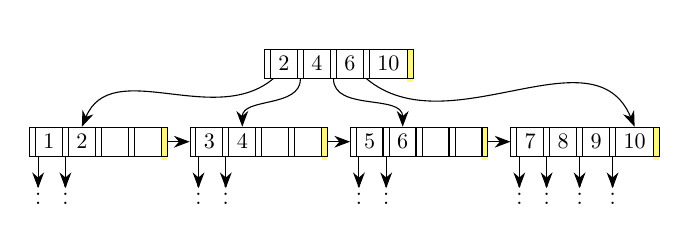
\begin{tikzpicture}[
		scale=0.8,
		transform shape,
		x=2em,
		node distance=0.5,
		treenode/.style={
			draw,
			rectangle split,
			rectangle split horizontal=true,
			rectangle split parts=9,
			rectangle split empty part width=-3mm,
			rectangle split part fill={
				none, none, none, none, none, none, none, none,
				yellow!50
			}
		}
	]
	% Nodes
	\node[treenode] (leaf1) {
		\nodepart{two}1\nodepart{three}
		\nodepart{four}2\nodepart{five}
		\nodepart{six}\phantom{0}\nodepart{seven}
		\nodepart{eight}\phantom{0}
	};
	\node[treenode, right=of leaf1] (leaf2) {
		\nodepart{two}3\nodepart{three}
		\nodepart{four}4\nodepart{five}
		\nodepart{six}\phantom{0}\nodepart{seven}
		\nodepart{eight}\phantom{0}
	};
	\node[treenode, right=of leaf2] (leaf3) {
		\nodepart{two}5\nodepart{three}
		\nodepart{four}6\nodepart{five}
		\nodepart{six}\phantom{0}\nodepart{seven}
		\nodepart{eight}\phantom{0}
	};
	\node[treenode, right=of leaf3] (leaf4) {
		\nodepart{two}7\nodepart{three}
		\nodepart{four}8\nodepart{five}
		\nodepart{six}9\nodepart{seven}
		\nodepart{eight}10
	};
	\coordinate (center) at ($ (leaf2) !.5! (leaf3) $);
	\node[treenode, above=1 of center] (root) {
		\nodepart{two}2\nodepart{three}
		\nodepart{four}4\nodepart{five}
		\nodepart{six}6\nodepart{seven}
		\nodepart{eight}10
	};
	% Connections
	\draw[->] (root.south west)++(0.2,0) to[out=220,in=67.5] (leaf1.four north);
	\draw[->] (root.three south) to[out=270,in=90] (leaf2.four north);
	\draw[->] (root.five south) to[out=270,in=90] (leaf3.four north);
	\draw[->] (root.seven south) to[out=320,in=112.5] (leaf4.eight north);
	\draw[->] (leaf1.east) -- (leaf2.west);
	\draw[->] (leaf2.east) -- (leaf3.west);
	\draw[->] (leaf3.east) -- (leaf4.west);
	% Data
	\foreach \i in {1,2,3,4} {
		\draw[->] (leaf\i.south west)++(0.2,0) -- ++(0, -0.5) node {$\vdots$};
		\draw[->] (leaf\i.three south) -- ++(0, -0.5) node {$\vdots$};
	}
	\draw[->] (leaf4.five south) -- ++(0, -0.5) node {$\vdots$};
	\draw[->] (leaf4.seven south) -- ++(0, -0.5) node {$\vdots$};
\end{tikzpicture}

	\end{figure}
\end{frame}


\subsection{FPGAs}

\begin{frame}
	\frametitle{FPGAs}
	\begin{itemize}
		\item Reconfigurable array of programmable logic elements
		\note[item] {
			Introduction classes only mentoin LUTs, but there's more available
		}
		\item Can implement niche accelerators cost effictively
		\begin{itemize}
			\item Alternative to custom silicon
			\item Flexibility to update as needed
			\note[item] {Used in some cellular modems for this reason}
			\note[item] {Silicon bugs are insanely costly}
			\note[item] {
				Pentium FDIV happened 5 years before I was born and I've still
				heard of it
			}
			\item Faster development cycle
			\note[item] {
				For those who enjoy ``moving fast and breaking things''
			}
		\end{itemize}
		\item Relatively low clock speeds save power
		\note[item] {
			Important in the age of nuclear-powered AI datacenters
		}
		\item Size of designs that can be implemented on one chip has increased
		over time
	\end{itemize}
\end{frame}


\begin{frame}
	\frametitle{Resource Multiplexing}
	\begin{columns}
		\column{0.47\linewidth}
		\begin{itemize}
			\item On a CPU, computation is multiplexed \emph{temporally}
			\item Instructions per clock cycle is limited
			\item Even with superscalar architectures, pipeline stages are a
			limiting factor
			\note[item] {
				Even if the five-stage pipeline isn't in vogue anymore, the
				concept still stands
			}
		\end{itemize}

		\column{0.5\linewidth}
		\begin{figure}
			\centering
			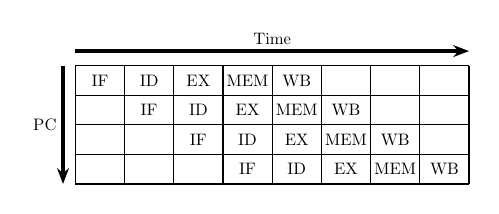
\begin{tikzpicture}[
		xscale=0.625,
		yscale=0.375,
		every node/.style={
			scale=0.6
		}
	]
	% Diagram
	\draw (1, 0) grid (9, -4);
	\foreach \i in {1,2,3,4} {
		\node at ({\i+0.5}, {0.5-\i}) {IF};
		\node at ({\i+1.5}, {0.5-\i}) {ID};
		\node at ({\i+2.5}, {0.5-\i}) {EX};
		\node at ({\i+3.5}, {0.5-\i}) {MEM};
		\node at ({\i+4.5}, {0.5-\i}) {WB};
	}
	% Axes
	\draw[->, very thick]
		(1, 0.5) to node[above] {Time} ++(8, 0);
	\draw[->, very thick]
		(0.75, 0) to node[left] {PC} ++(0, -4);
\end{tikzpicture}

			\caption{Generic CPU Pipeline}
		\end{figure}
	\end{columns}
\end{frame}


\begin{frame}
	\frametitle{Resource Multiplexing}
	\begin{columns}
		\column{0.47\linewidth}
		\begin{itemize}
			\item On an FPGA, computation is multiplexed \emph{spatially}
			\item All functional units can operate simultaneously
			\note[item]{
				This isn't to say that FPGAs don't have critical paths, but they
				floorplan is far more likely to become a bottleneck
			}
			\item FPGA fabric contains registers, memory, LUTs, and ALUs
			\note[item] {
				These aren't proper generic ALUs, but dedicated implementations
				of adders and other common arithmetic circuits.
			}
			\item Interconnect scarcity is also important
		\end{itemize}

		\column{0.5\linewidth}
		\begin{figure}
			\centering
			\includegraphics[width=\textwidth]{floorplan.png}
			\caption{Our Design's Floorplan}
		\end{figure}
	\end{columns}
\end{frame}


\subsection{HDLs \& HLS}

\begin{frame}
	\frametitle{Hardware Description Languages}
	\note[item] {Now for the downsides of FPGA design}
	\begin{columns}
		\column{0.47\linewidth}
		\begin{itemize}
			\item Different programming paradigm
			\item Learning curve is steep
			\item Pool of developers is small
			\item Limited abstraction
			\begin{itemize}
				\item Complex designs are difficult
			\end{itemize}
		\end{itemize}
		
		\column{0.5\linewidth}
		\lstinputlisting[language=verilog]{hdl.v}
	\end{columns}
\end{frame}


\begin{frame}
	\frametitle{High-Level Synthesis}
	\begin{itemize}
		\item HLS converts software programs into HDL designs
		\begin{itemize}
			\item \texttt{\#pragma}s are used to tweak HDL implemention
		\end{itemize}
		\item Can create parallel designs without needing to understand hardware
		\note[item] {
			Similar to how you can write good software without understanding how
			transistors work
		}
		\note[item] {
			Professor Krishnamurthy me
		}
		\item Automates interfacing with other hardware
		\note[item] {
			My design uses HBM and PCIe interfaces, but I never needed to touch
			either of those protocols
		}
		\note[item] {
			HDL IPs for those things surely exist, but connecting them properly
			is often non-trivial
		}
		\item Brings higher level of abstraction to FPGA design
	\end{itemize}

	\lstinputlisting[
		language=c,
		morekeywords={pragma},
		xleftmargin=0.2\textwidth
	]{hls.c}
\end{frame}


\section{Architecture}

\begin{frame}
	\frametitle{\todo{Title}}
	\todo{Content}
\end{frame}


\subsection{Trees}

\begin{frame}
	\frametitle{\todo{Title}}
	\todo{Content}
\end{frame}


\subsection{Memory}

\begin{frame}
	\frametitle{\todo{Title}}
	\todo{Content}
\end{frame}


\subsection{FPGA}

\begin{frame}
	\frametitle{\todo{Title}}
	\todo{Content}
\end{frame}


\section{Results}

\begin{frame}
	\frametitle{\todo{Title}}
	\todo{Content}
\end{frame}


\section{Conclusion}

\begin{frame}
	\frametitle{\todo{Title}}
	\begin{itemize}
		\item More FPGA parallelism is possible
		\begin{itemize}
			\item Multimodule, heterogeneous modules
		\end{itemize}
	\end{itemize}
\end{frame}


\begin{frame}
	\frametitle{References}
	\printbibliography
\end{frame}


\end{document}
